\section{Results}

We provide extensive simulation and experimental data and their interpretation,
supporting that the proposed analog signal generator works as intended.

\vspace{-1em}
\subsection{Simulation}
\vspace{-1em}

We perform a realistic simulation with a second-order low-pass filter we came up
with in Section~\ref{ssec:second}. One of the important aspects of this design
is the selection of the op-amp. In order to keep the common-mode voltage at
$0$\unit{\volt} we choose the op-amps as CMOS type. One such op-amp is
\texttt{OP292}~\cite{op292}, which is used in this simulation.

The PWM signal generated by Teensy~\cite{teensy} is simulated exactly with a
carrier frequency of $36.6$\unit{\kilo\hertz} modulating the signal \[
V_{\text{pwm}} = \nicefrac{3.3}{2} + \nicefrac{3.3}{2}\sin{(2\pi 90 t)}.\]
Finally, the impedance of the load (PI's controller) is read off from its
datasheet and inserted as a $100$\unit{\kilo\ohm} resistance. The circuit that
is simulated using LTSpice~\cite{ltspice} is presented in
Figure~\ref{fig:real_sig_gen}.

\begin{figure}[htb] 
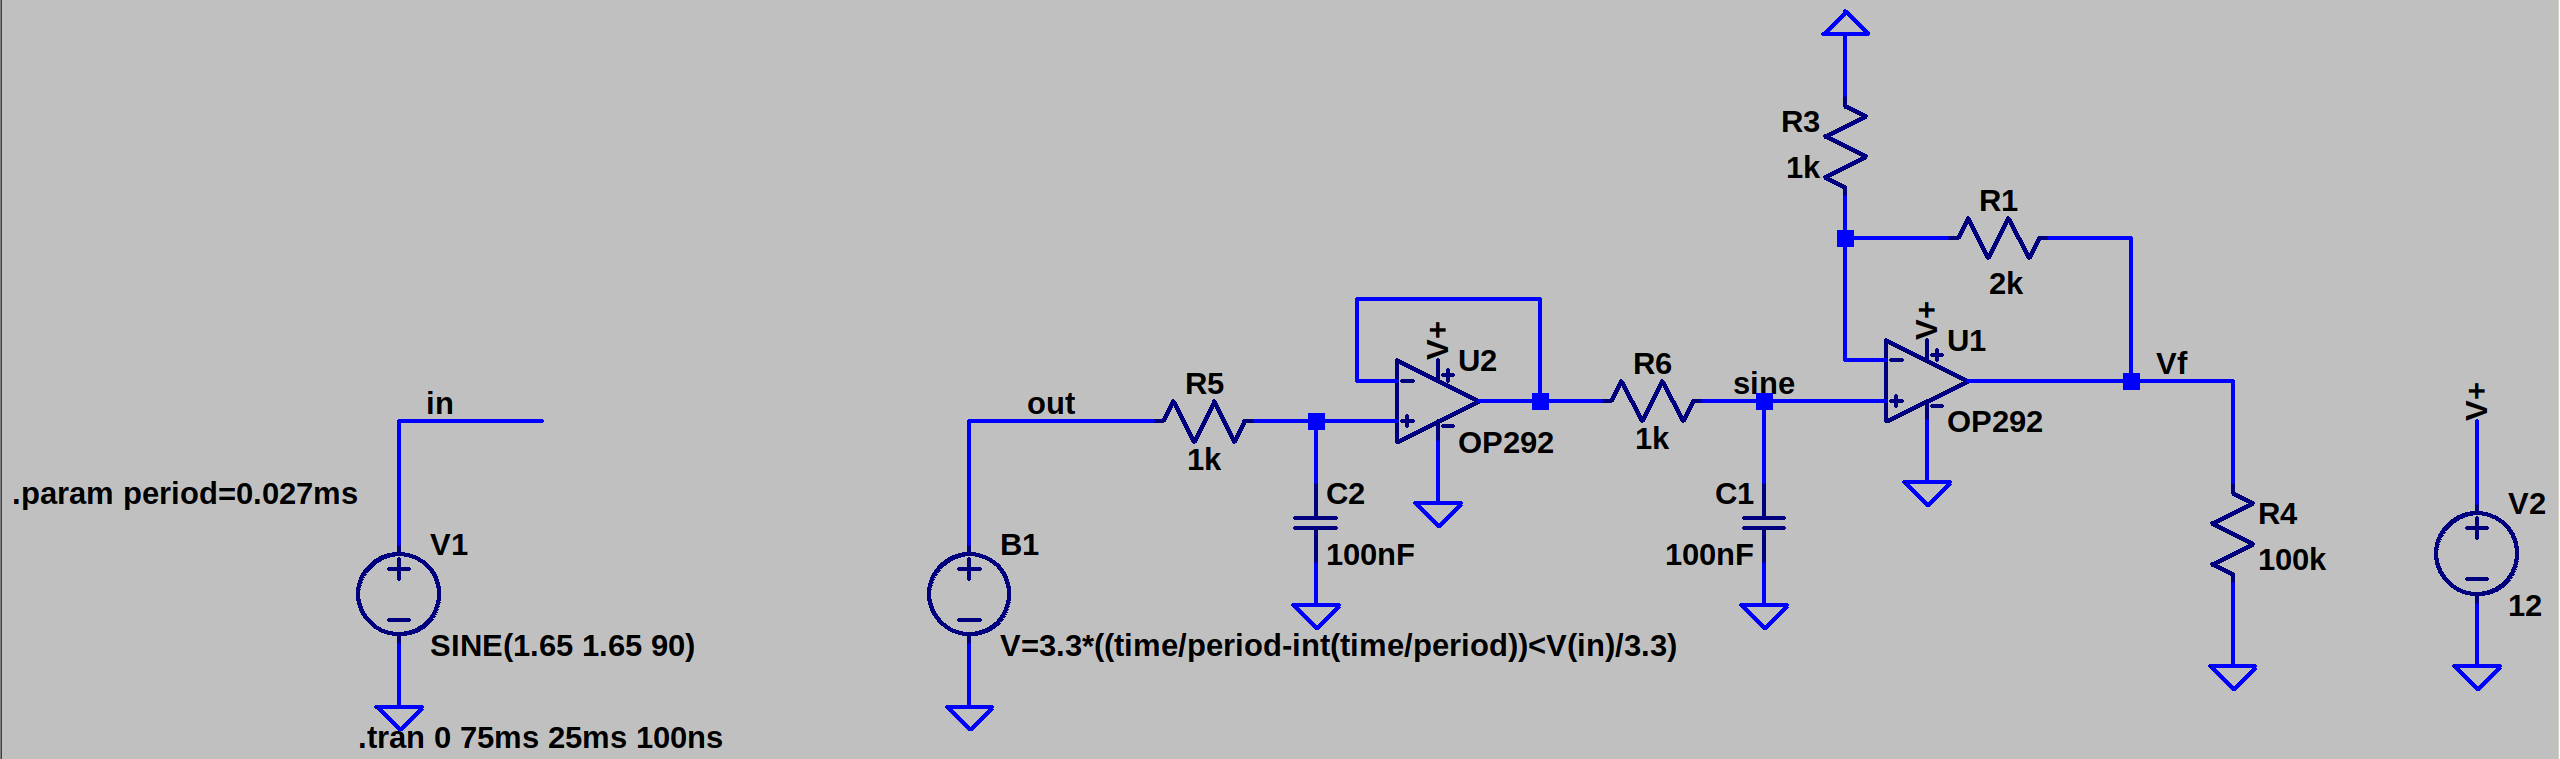
\includegraphics[width=8cm]{./figures/circuit.png}
\caption{The signal generator circuit in LTSpice} 
\label{fig:real_sig_gen}
\end{figure}

The simulation generates the relevant voltage responses, provided in
Figure~\ref{fig:response}. The top plot shows the PWM signal generated by Teensy
modulating a sine-wave at $90$\unit{\hertz} frequency. The individual plots in
the middle show the output of the first (cyan) and the second (purple) RC
low-pass filters ($v_f$ and $v_i$, respectively) that extract the modulated
signal from its PWM representation. Finally, the last plot shows the amplified
signal (gain: $3$) through the op-amp \texttt{OP292}. This signal is ready to be
sent to the PI controller.

\begin{figure}[t]
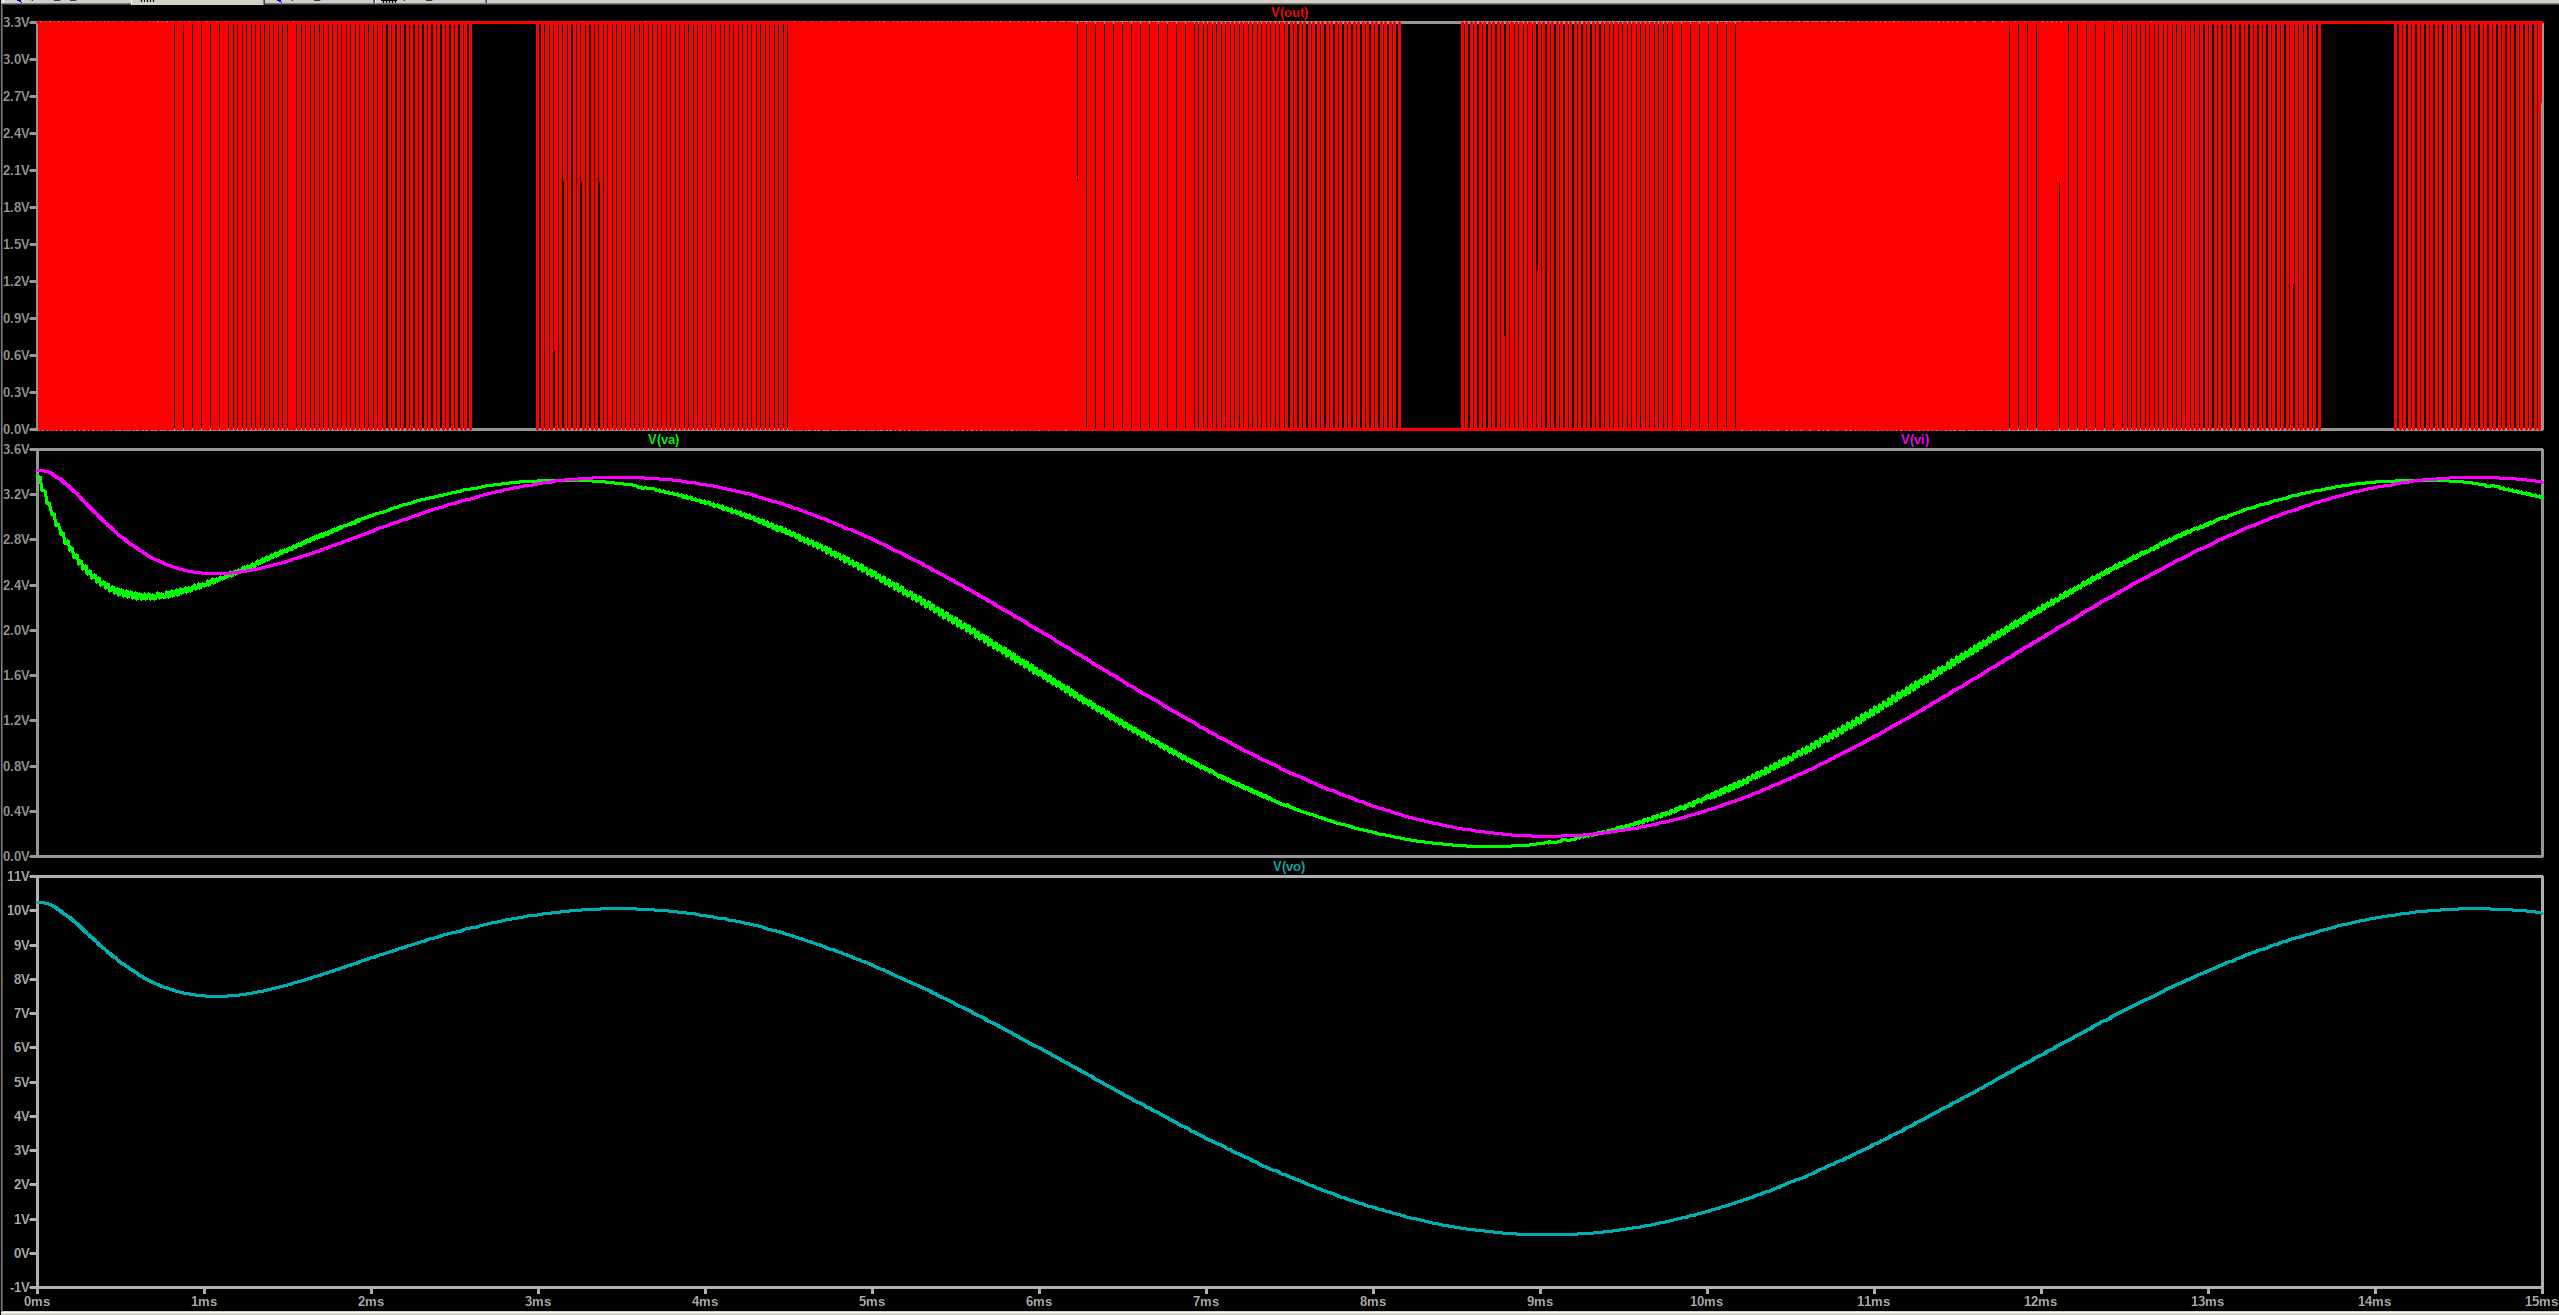
\includegraphics[width=0.5\textwidth]{./figures/pwm_filtered_one_two_final_signal.png}
\caption{The response from the simulation for one full period.} 
\label{fig:response}
\end{figure}


\vspace{-1em}
\subsection{Experiment}
\vspace{-1em}

The design is implemented on a simple setup on my table top by lighting two red
LEDs, first one using the filtered PWM and the second using the amplified
signal, both obtained using the circuit in Section~\ref{ssec:second}.

\begin{figure}[t]
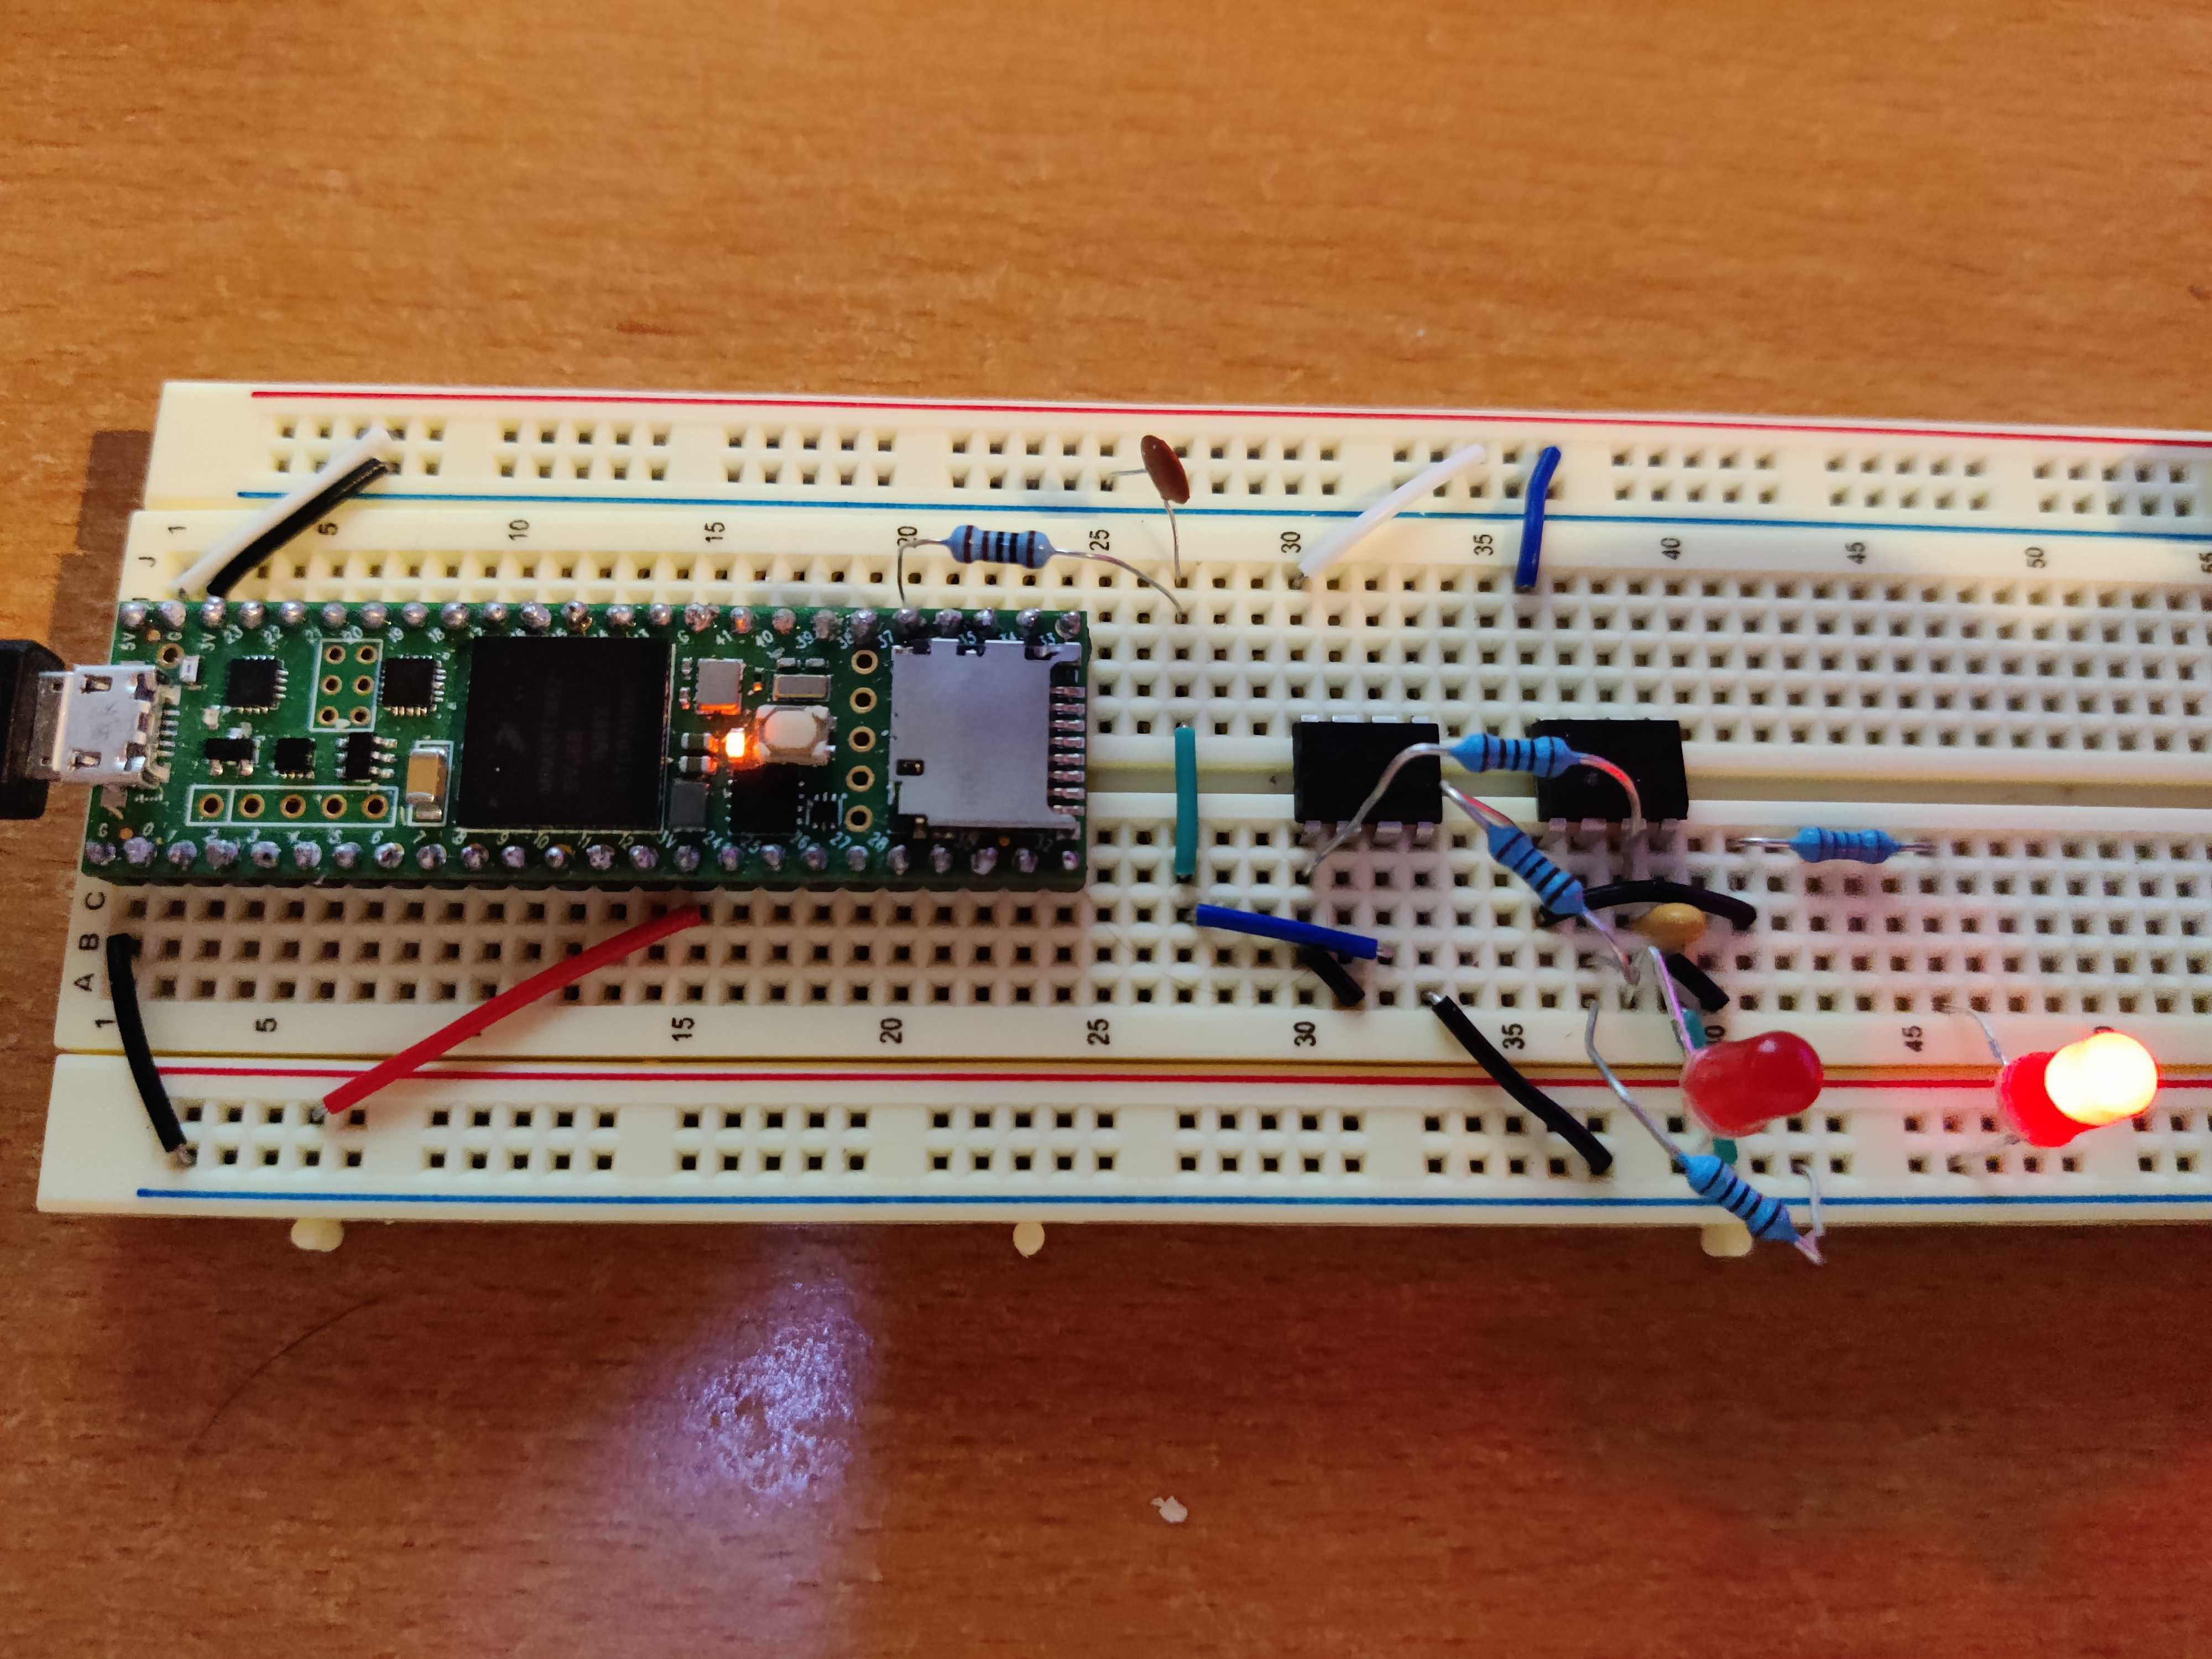
\includegraphics[width=0.5\textwidth]{./figures/prototype.jpg}
\caption{Prototype working on a LED} 
\label{fig:exp}
\end{figure}

We will perform a final verification on the real piezoelectric system early next
week, recording the input signal properly using an oscilloscope.
